\chapter{入门以后}

站在上一章的入门基础之上,本章我将介绍一些更为有趣的东西。这些貌似“高级”的技术其实也不复杂,
无非是再多认识几个命令和环境罢了。

\section{插入图片}

\begin{codeblock}[.9]
\begin{latexcode}
  \documentclass{article}
  
  \usepackage{graphicx}
  \graphicspath{{./figs/}{./}}
  
  \begin{document}
  
\includegraphics[width=5cm]{tux}
  \end{document}
\end{latexcode}
\end{codeblock}

怎么样,能看明白吗?插入图片用到了三个新命令:

\begin{enumerate}
\item \ltx{\usepackage{graphicx}}, 这是在说「我要用到一个名字叫 graphicx 的package(宏包)」。
  这很类似于我们C编程时常用的\cinline{#include<stdio.h>}。\ltx{\include-graphics{}}就
  是这个宏包提供的命令之一。想详细了解 graphicx的话,你可以打开一个命令终端,敲命
  令:\texttt{texdoc graphicx}。\texttt{texdoc}是TeXLive提供的专门用来看各种宏包手册的小工
  具。你可以通过\texttt{texdoc -h}命令来粗略了解它的用法。
\item \ltx{\graphicspath{{./figs/}{./}}}, 显然这是在指明graphics(图片)所在的path(路径,位
  置),也就是说,当你编译的时候,\LaTeX{}会到你指定的地方去找要插入的图片。在这里,我指定
  了两个地方:
  \begin{enumerate}
  \item \texttt{./figs/},当前目录下的\texttt{figs}目录。如果在这里没有找到,那么就去下面的
    目录里接着找;
  \item \texttt{./},也就是当前目录。如果在这个目录里还是没找到想插入的图片,那么编译器就要
    报错了。
  \end{enumerate}
\item \ltx{
\includegraphics[width=5cm]{tux}},这显然就是在插入图片了。
  \begin{enumerate}
  \item 图片的名字叫 \texttt{tux.pdf}, 后缀(\texttt{.pdf})可以被省略掉。显
    然 \texttt{tux.pdf} 应该被存放在 \texttt{./} 或者 \texttt{./figs/} 中,才能被找到。我喜
    欢PDF图片,因为它可以自由缩放。你当然可以插入jpeg、png图片。
  \item 宽度是5cm,也可以是相对宽度,比如 \ltx{[width=.5\linewidth]} 就表示宽度等于0.5倍的行宽。
  \end{enumerate}
\end{enumerate}

如果你希望图片“居中”摆放,那自然是要用到 center 了:

\begin{codeblock}[.9]
\begin{latexcode}
  \documentclass{article}
  
  \usepackage{graphicx}
  \graphicspath{{./figs/}{./}}
  
  \begin{document}
  \begin{center}
    
\includegraphics[width=5cm]{tux}
  \end{center}
  \end{document}
\end{latexcode}
\end{codeblock}

编译后的效果大致就是这样,居中,5cm宽。

\begin{center}
  
\includegraphics[width=5cm]{tux}
\end{center}

\subsection{Figure环境}
\label{sec:figure}

“哎,似乎应该加上图片说明吧?比如,【图1: Linux图标】?” 这个容易,只要用到一个新的
environment,叫figure。

\Ctrlcc{e} figure \Ctrl{j},mini buffer提示:
\begin{enumerate}
\item[] \texttt{(Optional) Float position:}
\end{enumerate}

这是在问你图片放在那里比较好啊?是靠上?还是靠下?还是懒得操心?如果没概念,那还是让LaTeX
来决定吧,\Ctrl{j}, mini buffer 提示:

\begin{enumerate}
\item[] \texttt{Caption:}
\end{enumerate}

这是在提示你输入图片的说明文字。那么输入:

\begin{enumerate}
\item[] \texttt{Linux logo}
\end{enumerate}

mini buffer 提示:

\begin{enumerate}
\item[] \texttt{Center? (y or n):} 
\end{enumerate}

当然选:

\begin{enumerate}
\item[] \texttt{y}
\end{enumerate}

mini buffer 提示:

\begin{enumerate}
\item[] \texttt{Label: fig:}
\end{enumerate}

这是要你给图片打个标签,以后方便索引到它。那么就给个标签:

\begin{enumerate}
\item[] \texttt{linux-logo}
\end{enumerate}

于是得到:

\begin{codeblock}[.9]
\begin{latexcode}
  \documentclass{article}
  
  \usepackage{graphicx}
  \graphicspath{{./figs/}{./}}
  
  \begin{document}
  \begin{figure}
    \centering
    
    \caption{Linux logo}
    \label{fig:linux-logo}
  \end{figure}
  \end{document}
\end{latexcode}
\end{codeblock}

现在你建立了一个完美的图片环境,别忘了把图片放进去。当然放在第9行:

\begin{codeblock}[.9]
\begin{latexcode}
  \documentclass{article}
  
  \usepackage{graphicx}
  \graphicspath{{./figs/}{./}}
  
  \begin{document}
  \begin{figure}
    \centering
    
\includegraphics[width=5cm]{tux}
    \caption{Linux logo}
    \label{fig:linux-logo}
  \end{figure}
  \end{document}
\end{latexcode}
\end{codeblock}

编译后的效果如图\ref{fig:linux-logo}所示。

\subsection{\tbs{label\{\}}和 \tbs{ref\{\}}的用法}
\label{sec:label}

\ltx|\label{}|到底怎么用?来看下面的例子就明白了。

\begin{codeblock}[.9]
\begin{latexcode}
  \documentclass{article}
  
  \usepackage{graphicx}
  \graphicspath{{./figs/}{./}}
  
  \begin{document}
  \begin{figure}
    \centering
    
\includegraphics[width=5cm]{tux}
    \caption{Linux logo}
    \label{fig:linux-logo}
  \end{figure}

  Figure~\ref{fig:linux-logo} is the famous Linux Tux!
  图\ref{fig:linux-logo}所示就是大名鼎鼎的Linux吉祥物!
  \end{document}
\end{latexcode}
\end{codeblock}

编译一下,看看效果吧:

\begin{figure}
  \centering
  
\includegraphics[width=5cm]{tux}
  \caption{Linux logo}
  \label{fig:linux-logo}
\end{figure}

\begin{center}
  \begin{minipage}{.6\linewidth}
    \hrule    \vskip 1ex
    Figure~\ref{fig:linux-logo} is the famous Linux Tux! 图\ref{fig:linux-logo}所示就是大名
    鼎鼎的Linux吉祥物!
    \vskip 1ex    \hrule
  \end{minipage}
\end{center}

\ltx{\label{}} 和 \ltx{\ref{}} 总是配合使用的,一个用来打标签,另一个用来找标签。而且这
两个命令可以被用在任何你需要的地方,非常方便。比如,

\begin{codeblock}[.9]
\begin{latexcode}
  % 本文的第一章标题
  \chapter{工欲善其事,必先利其器}
  \label{cha:pre-requisite}   % 章标签

  % 本文中的某张表格
  \begin{table}[!htbp]
    \centering
    \caption{常用快捷键}\label{tab:keys}  % 表格标签
    \begin{tabu*}to .5\textwidth {X[r]|X[l]}
      \hline
      \rowfont[c]{\bfseries}快捷键&功用\\\hline
      \Cj{}&换行带缩进\\
      \Cc\Cm{}&输入Macro\\
      \Cc\Cs{}&新起一个章节\\
      \Cc\Ce{}&新起一个环境\\
      \MEnter{}&换行带{\verb|\item|}\\\hline
    \end{tabu*}
  \end{table}

  % 在文中某处有这样一行
  最基本的Emacs快捷键(大多以\Cx{}开头)\label{p:keys} % 任意标签

  %%% 下面让我们来使用(索引)上面的标签
  
  \begin{enumerate}
  \item 本文的第~\ref{cha:pre-requisite}章介绍了一个简单、% 索引某章
    高效的工作环境;
  \item 在表~\ref{tab:keys}中列出了几个最常用的快捷键; % 索引某表
  \item 在第~\pageref{p:keys}页列出了更多的快捷键。    % 索引某页
  \end{enumerate}
\end{latexcode}
\end{codeblock}

上述代码就可以生成如下的效果,不仅数字是正确的,而且它们都是hyperlink,用鼠标点一下试试。

\begin{enumerate}
\item 本文的第\ref{cha:pre-requisite}章介绍了一个简单、高效的工作环境;
\item 在表\ref{tab:keys}中列出了几个最常用的快捷键;
\item 在第\pageref{p:keys}页列出了更多的快捷键。
\end{enumerate}

\subsubsection*{快捷地插入标签和索引}

插入标签和索引也是有快捷键的。\Ctrl{c}\biolinumKeyGlyph{braceleft}就是要插入标签,mini
buffer提示:

\begin{enumerate}
\item[] \texttt{Label: cha:}
\end{enumerate}

如果你不是要插入章标签,那么可以把\texttt{cha}改成其它你认为合适的字符。通常Emacs会根据光
标所在的环境给出不同的提示,如果光标在

\begin{itemize}
\item Figure里,它就提示\texttt{fig:};
\item Table里,它就提示\texttt{tab:};
\item 正文中其它什么地方,它就提示 \texttt{cha:}或者 \texttt{sec:}。
\end{itemize}

现在,在提示下输入一个简短而好记的标签名称,以便后面可以轻松找到它。

要插入索引(\ltx{\ref{}})的话,敲 \Ctrl{c}\biolinumKeyGlyph{braceright},mini buffer 提示:

\begin{itemize}
\item[] \texttt{SELECT A REFERENCE FORMAT}
\item[] \verb'[^M]  \ref'
\item[] \verb'[p]   \pageref' 
\end{itemize}

这是让你选择索引格式,如果想索引某页的话,就选\texttt{[p]}。其它任何情况,都选
择\verb'[^M]',也就是敲\LKeyEnter{}直接回车。根据你的选择,Emacs会弹出新的buffer,方便你找
到要引用的标签。

\section{数学公式}
\label{sec:math}

举个简单的例子吧:

\begin{codeblock}[.9]
\begin{latexcode}
  \documentclass{article}
  \begin{document}
  This is a simple math example: $c^2=a^2+b^2$
  \end{document}
\end{latexcode}
\end{codeblock}

结果是这样:

\begin{itemize}
\item[] This is a simple math example: $c^2=a^2+b^2$
\end{itemize}

美元符号(\verb'$')在 \LaTeX{}里面是特殊字符。夹在两个美元符号之间的东西,会被当做数学公式来排版。
如果想让数学公式独占一行的话,就用双美元符号(\verb'$$'),比如,
$$(1+x)^n=\sum_{k=0}^n\binom{n}{k}x^k$$
就是\verb'$$(1+x)^n=\sum_{k=0}^n\binom{n}{k}x^k$$'的输出结果。还不难看懂吧?

\begin{itemize}
\item \verb'\sum' $\Rightarrow\sum$
\item \verb'\binom{n}{k}' $\Rightarrow\binom{n}{k}$
\item 下划线(\texttt{\_})后面跟下标,如果下标不止一个字符,那么就要用花括号
  (\texttt{\{\}})括起来。比如,\verb'A_1 + A_{100}' $\Rightarrow{}A_1 + A_{100}$;
\item 上箭头(\verb'^')后面跟上标,用法和下划线一样。比如,\verb'2^2 \times 2^{32}'
  $\Rightarrow$ $2^2\times{}2^{32}$。 
\end{itemize}

那么,去哪里找这些数学符号呢?很简单,Google一下“latex math”,就什么都有了。“天啊,谁能记住
那么多数学符号啊?!”。\LaTeX{}的数学排版功能博大精深,各式各样的数学符号、怪异字符无所不及,
当然用不着都记住。你只要记住上面我们提到的几条,应该就足以应付毕业论文了。如果你要经常对付
复杂数学公式的话,那么最好把《The \LaTeX{} Companion》\cite{Goossens94a}这本书的第八章
(Higher Mathematics)打印下来放在手边,随用随查就好了。Google一下“latex math chapter 8”。

\section{插入程序代码}
\label{sec:code}

\begin{figure}
  \centering
\begin{minipage}[t]{.45\linewidth}
  代码:
  \begin{center}
    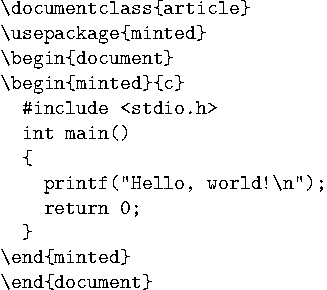
\includegraphics[width=\textwidth]{code}
  \end{center}
\end{minipage}
\hfill\vline\hfill
\begin{minipage}[t]{.45\linewidth}
  效果:
  \vspace{4.6em}
  \begin{minted}[baselinestretch=1,xleftmargin=0em]{c}
    #include <stdio.h>
    int main()
    {
      printf ("Hello, world!\n");
      return 0;
    }
  \end{minted}
\end{minipage}
  \caption{插入代码示例}\label{fig:code}
\end{figure}

还是从一个小例子开始吧,如图\ref{fig:code}所示,插入代码首先
要\ltx{\usepackage{minted}}。minted是用于美化代码排版的\LaTeX{}宏包,有了它,你可以把几乎
所有编程语言的代码排版得像你们老师那样道貌岸然,而且是彩色的。不过,对于毕业论文来说,还是
采用黑白排版比较好。彩色排版如果黑白打印,效果就很模糊了。当然你可以选择彩色打印,但那很费
钱啊。

想详细了解minted的用法,就:\texttt{texdoc minted}。minted宏包提供了一个新环境,就
叫minted ,把你的程序放在 \ltx|\begin{minted}|和\ltx|\end{minted}|之间就行
了。\ltx|\begin{minted}|后面的 \verb'{c}'当然是说,插入的程序是用C语言写的。
  
怎么?程序太长,拷贝进来太麻烦?那么可以这样:

\begin{codeblock}[.9]
\begin{latexcode}
  \documentclass{article}
  \usepackage{minted}
  \begin{document}
  
  \inputminted{c}{hello.c}
  
  \end{document}
\end{latexcode}
\end{codeblock}

简单吧?\texttt{hello.c} 当然要和你的 \TeX{} 文件在同一个目录下,否则你要指明详细路径。

minted宏包提供了丰富的命令,可以支持数十种编程语言,后台调用强大的pygments来打扮你的程序
代码,可以把程序以各种你能想到的方式排版出来。当然,使用 minted 的前提条件是,系统里已经安
装好了python和pygments。这一点在minted的手册里已经说得很清楚了。关于强大的pygments,
你该去它的网站看看:\url{http://pygments.org/}。

\section{处理中文}
\label{sec:cn}

如果你的Emacs配置和我的一样,那么输入中文就是“piece of cake”,当然你得安装了中文输入法,我
用的是fcitx\footnote{\url{https://fcitx-im.org/wiki/Fcitx}},挺好用的。

现在,打开一个全新的\texttt{tex}文件,比如\texttt{hello.tex},在里面写\texttt{ctexart},然
后敲\LKeyTab{}(TAB)键,一个现成的\LaTeX{}文件模板立时会展现在你的面前。这个模版里有你写一篇漂
亮中文文章所需要的一切。光标就停在 \ltx|\title{}| 的花括号里,那么就开始用中文填空
吧。重点就是第一句:

\begin{latexcode}
\documentclass[scheme=chinese]{ctexart}
\end{latexcode}

也就是说,只要直接采用\texttt{CTeX}提供的\texttt{ctexart class},中文问题就不需要我们操心
了。


%%% Local Variables:
%%% mode: latex
%%% TeX-master: "../example"
%%% End:
